Cette section vise à observer l'impact du niveau de reconstruction des flux quand l'opérateur de diffusion est couplé à un autre opérateur. 
L'équation de diffusion est remplacée par l'équation de Nagumo (voir \ref{par:analyser_operateurs_nagumo}) qui ajoute un terme de réaction. 
Des ondes progressives sont solution de cette équation, le schéma numérique donc doit être en mesure de suivre la dynamique du front d'onde.

\subsubsection{Résumé de l'expérience}
L'expérience à été réalisée dans des conditions similaires à l'expérience numérique \ref{par:contrib_imex}. 
C'est à dire :
\begin{itemize}
    \item[$\diamond$] Profil de l'onde propagative comme état initial.
    \item[$\diamond$] Domaine étendu avec conditions de Neumann aux limites pour limiter les effets de bord
\end{itemize}
La seule différence majeur réside dans le remplacement de la méthode Runge et Kutta ImEx par un schéma de splitting avec une méthode stabilisée explicite pour la diffusion (ROCK 2 \cite{AbdulleMedovikov2001}).
Ce choix découle de la nécessité d'éviter toute inversion de système linéaires lorsque l'on reconstruit les flux à partir d'approximation 
fines car l’implémentation prendrait actuellement trop de temps.


\subsubsection{Résultats de l'expérience}
Les résultats de l'expérience sont donnés en figure \ref{}
\begin{figure}[h!]
    \centering
    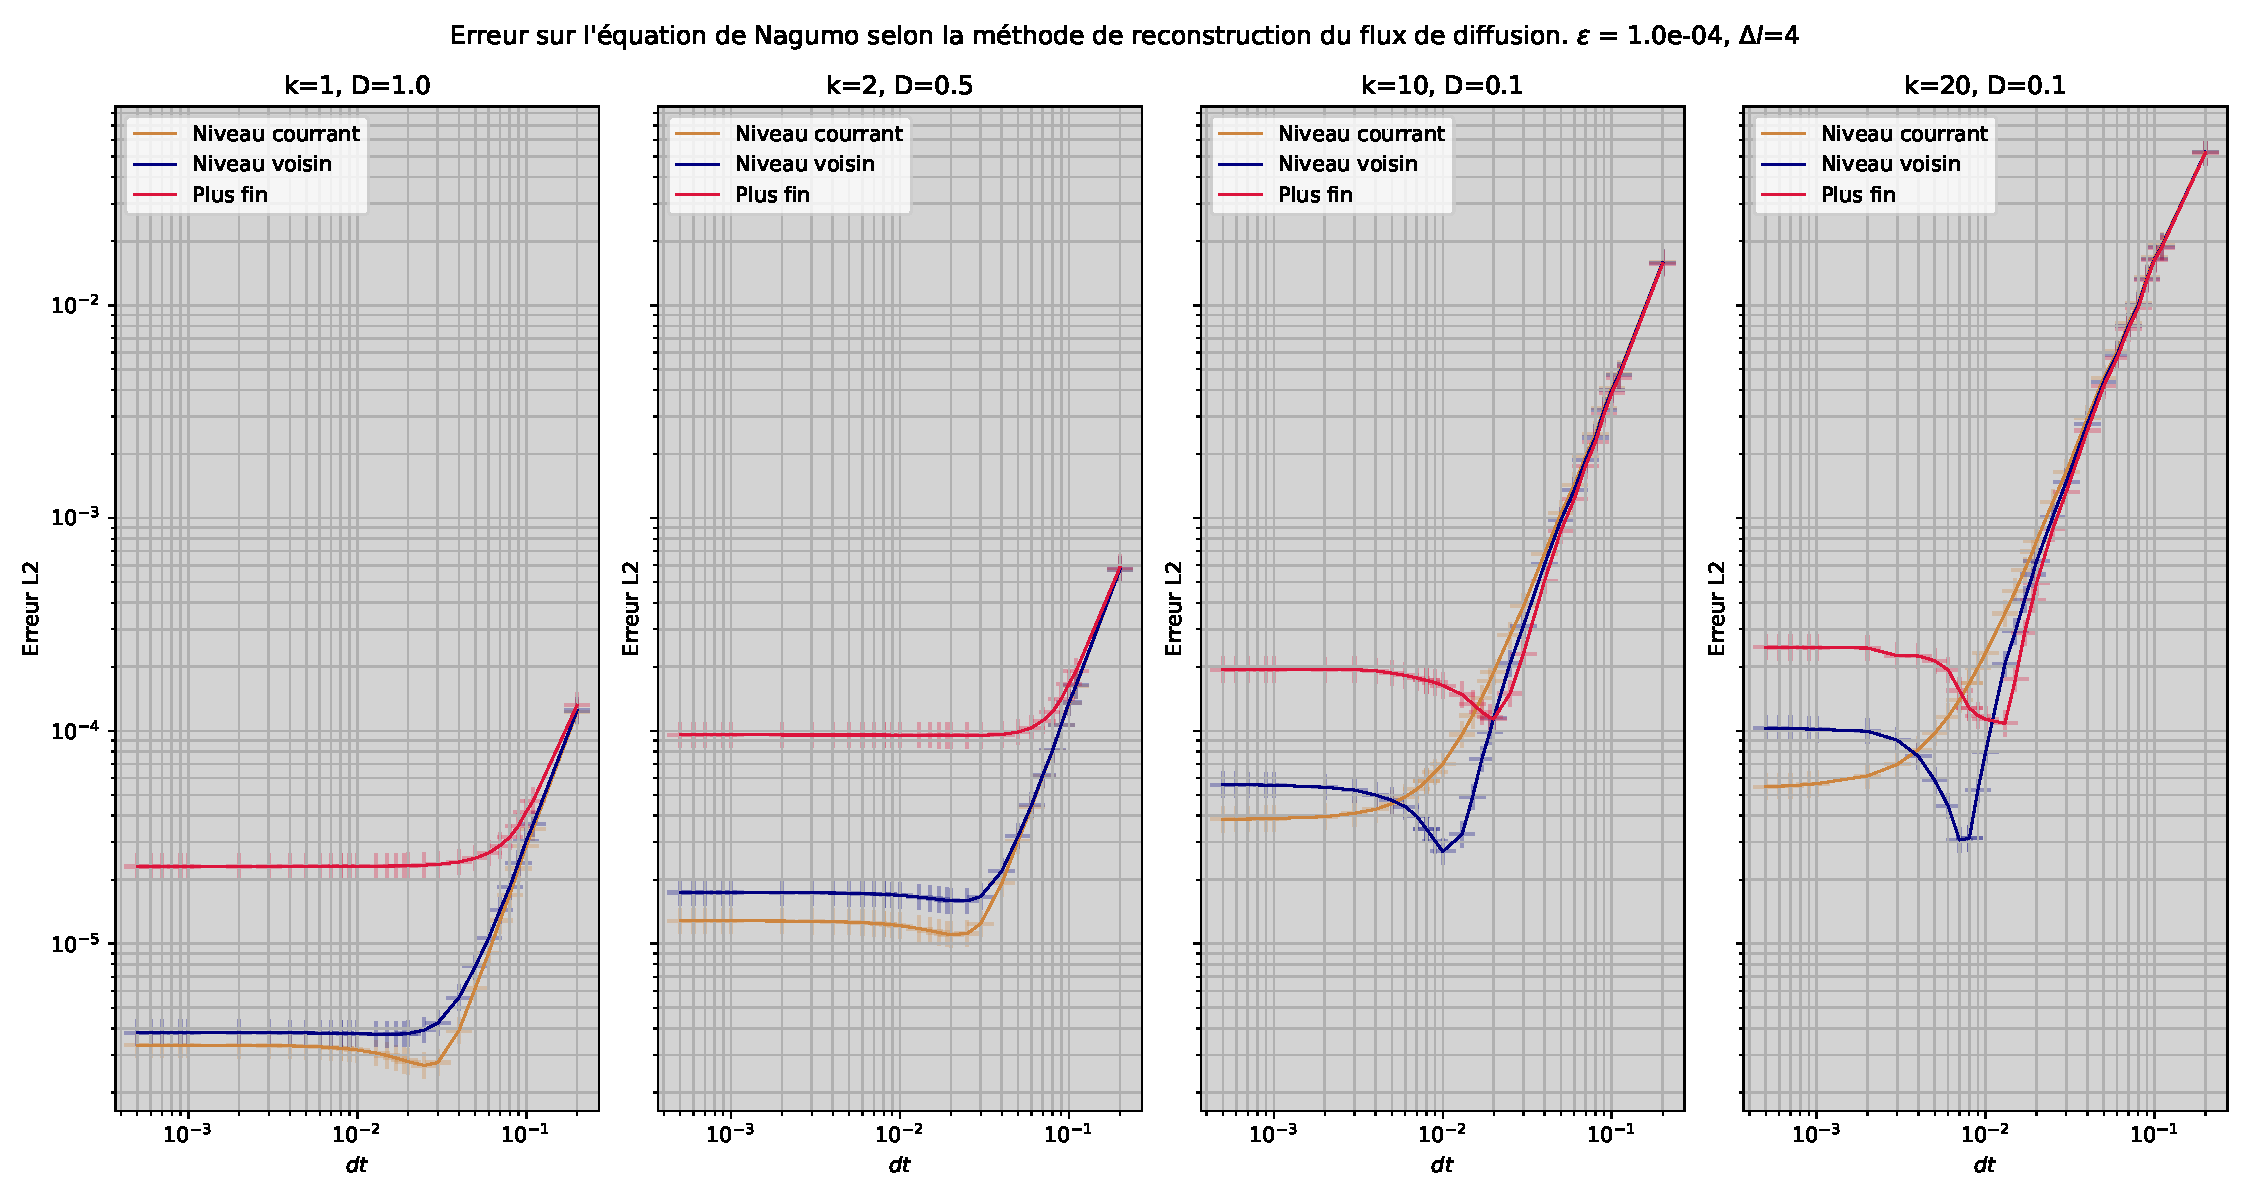
\includegraphics[width=\textwidth]{media/4_travail/3/flux_reconstruction_method_nagumo.pdf}
    \caption{Courbes de convergence de chaque méthode d'AMR pour différents paramètres de l'équation. Plus $k$ est élevé, plus le profil de l'onde est raide et plus la réaction domine. La célérité de l'onde est néanmoins identique pour chaque jeu de paramètres puisque le produit $kD$ reste constant d'une expérience à l'autre.}
    \label{fig:flux_reconstruction_nagumo}
\end{figure}